% Heimrouter von hinten: Ab Overlay 2 wird sichtbar, welche Anschlüsse zu Router und Switch gehören.
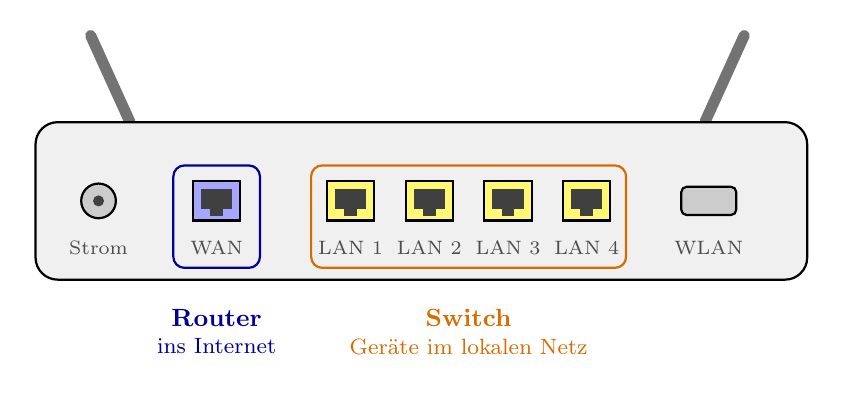
\begin{tikzpicture}[
        antenne/.style={line width=4pt, line cap=round, black!55},
        bereich/.style={draw, thick, rounded corners=4pt, inner sep=5pt},
        rolle/.style={font=\small\bfseries, align=center},
        portname/.style={font=\scriptsize, black!70},
        pics/rj45/.style={code={
            % Netzwerkbuchse: Rahmen mit Rastnase unten
            \draw[thick, fill=#1] (-0.3,-0.25) rectangle (0.3,0.25);
            \fill[black!75] (-0.2,0.15) rectangle (0.2,-0.1);
            \fill[black!75] (-0.08,-0.1) rectangle (0.08,-0.19);
        }}
    ]
    % Feste Grösse, damit die Folie beim Einblenden der Rollen nicht springt
    \useasboundingbox (-4.7,-2.4) rectangle (5.3,2.2);
    % Antennen
    \draw[antenne] (-3.4,1.0) -- (-3.9,2.1);
    \draw[antenne] (3.9,1.0) -- (4.4,2.1);
    % Gehäuse
    \draw[thick, fill=black!6, rounded corners=8pt] (-4.6,-1.0) rectangle (5.2,1.0);
    % Stromanschluss
    \draw[thick, fill=black!20] (-3.8,0) circle (0.22);
    \fill[black!75] (-3.8,0) circle (0.07);
    \node[portname] at (-3.8,-0.6) {Strom};
    % WAN-Anschluss
    \pic at (-2.3,0) {rj45=blue!35};
    \node[portname] at (-2.3,-0.6) {WAN};
    % Vier LAN-Anschlüsse
    \foreach \x/\n in {-0.6/1, 0.4/2, 1.4/3, 2.4/4} {
        \pic at (\x,0) {rj45=yellow!55};
        \node[portname] at (\x,-0.6) {LAN \n};
    }
    % WLAN-Taste
    \draw[thick, fill=black!20, rounded corners=2pt] (3.6,-0.18) rectangle (4.3,0.18);
    \node[portname] at (3.95,-0.6) {WLAN};
    % Rollen erst nach \pause auf der Folie einblenden
    \only<2->{
        \draw[bereich, blue!60!black] (-2.85,-0.85) rectangle (-1.75,0.45);
        \draw[bereich, orange!85!black] (-1.1,-0.85) rectangle (2.9,0.45);
        \node[rolle, blue!60!black, anchor=north] at (-2.3,-1.25) {Router\\[-1pt]\footnotesize\mdseries ins Internet};
        \node[rolle, orange!85!black, anchor=north] at (0.9,-1.25) {Switch\\[-1pt]\footnotesize\mdseries Geräte im lokalen Netz};
    }
\end{tikzpicture}
